\Section{Motivation}

% Bring in the issues that our approach can address
% Describe them as problems in current simulation/emulation systems
Software defined networking (SDN) centralizes and simplifies control of network management,
and has been increasingly adopted in data centers and internet exchange points~\cite{B4, Meridian, SDX}.
%Software defined networking (SDN) technology separate the network control logic of the network from
%the distributed hardware that implementing the forwarding behaviors.
Similar to traditional computer network systems, it is crucial to perform appropriate testing and evaluation of
SDN-based applications before deploying on a real system.

Researchers in the simulation community have extended various existing network simulators to support SDN capability~\cite{S3F, NS3, OPNET}.
To improve experimental fidelity, researchers have also developed network emulation testbeds
(e.g., Mininet~\cite{Mininet}) that utilize Linux containers over shared hardware resources and
real network stack to run high-fidelity SDN experiments.
However, container-based emulators cannot reproduce the correct behavior of a real network
with a large network topology and high traffic load because of the limited underlying physical resources.
For example, on a commodity machine with 2.98 GHz CPU, 4 GB RAM, and 3 Gbps internal bandwidth,
Mininet can only emulate a network up to 30 hosts, each with a 100 MHz CPU, 100 MB RAM and connected by 100 Mbps links~\cite{ReproNetExprCBE}.
Therefore, increasing SDN testbed scalability and speed without losing the desired fidelity is essential.

% State our idea
In this paper, we present a model abstraction technique to transform an SDN-based network model to a ``one-big-switch'' network model.
This technique is useful if users only care about the end-to-end behavior rather than
the details within the network, such as hop-by-hop routing, or table lookup on each single switch.
For example, users may want to simulate a large-scale complex network of networks consisting of traditional TCP/IP networks,
SDN networks, industry control communication networks, etc.
The SDN components in this scenario may not be the focus, and thus maintaining only the end-to-end behavior is sufficient for running the hybrid experiment.
Our technique is also useful for real-time network simulation, in which models must be executed
no slower than the wall-clock time in order to interact with real implementations of network protocols and applications.
Failing to do so may result in temporal faults, i.e., the simulation fails to process events before the designated deadlines
required by the emulation or physical components. 
In addition, industrial collaborators may not want to disclose the details of their production network
(e.g., topology, routing, middle-box location and functionality) to modelers for privacy and security concerns.
They can use our model abstraction techniques on the target network and share the resulting ``one-big-switch'' model.

We develop a three-step approach to transform an SDN network to a big OpenFlow switch based network,
while still preserving the network forwarding logic equivalence.
The high-level idea is illustrated in Figure~\ref{OBS:Fig:BigSimOverview},
and the details are discussed in Section~\ref{OBS:Sec:Design}.
Our approach reduces the SDN network to a big-switch-based network to improve the scalability of SDN simulation or emulation.

\begin{figure}[t]
    \centering
    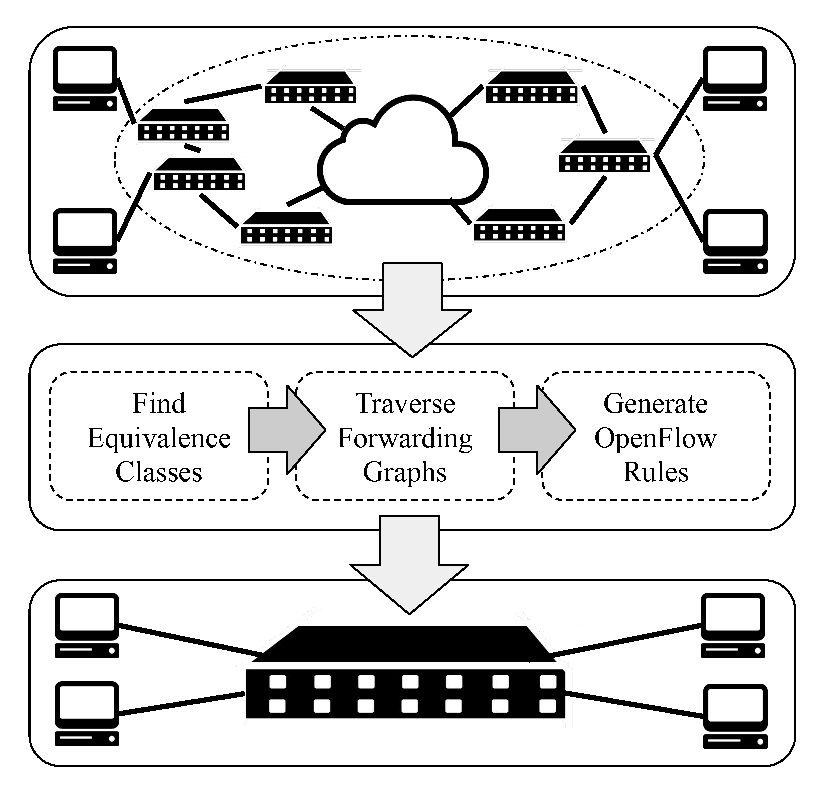
\includegraphics[width=0.9\textwidth]{OneBigSwitch/figures/BigSimOverview.eps}
    \caption[One Big Switch Abstraction Overview]{Transforming an SDN network to a
    big OpenFlow switch based network while preserving the network forwarding logic equivalence.}
    \label{OBS:Fig:BigSimOverview}
\end{figure}

The reduction in the number of switches and the number of rules significantly enhances the testbed scalability and reduces the experiment running time.
For example, after abstracting a tree-topology network of depth 4 and fanout 3,
the total number of switches required to simulate is reduced from 40 to 1, and the number of rules existed in the SDN network is reduced by 89\%.
The big-switch based network model can save about
75\% to 85\% simulation execution time as compared to simulating the original network.
We can also reuse the abstracted network model.
For example, after one complete experimental run of a complex network,
users can abstract (possibly part of) the network, and reproduce the simulation results with
a much simpler configuration, including link connectivity and flow tables.
We can partition a large-scale network model, and abstract each partition in parallel.
By combining those abstracted network models, a testing platform with limited hardware resources
now can afford such network simulation/emulation experiments.
As the network state evolves, the abstracted big-switch model may also need to be frequently updated.
Our approach is lightweight. For example, we can reduce 50,000+ rules in a large tree-topology network
to 5,000+ rules in a big-switch-based network in three seconds, 
while still preserving the network forwarding rule equivalence.
In addition, our approach allows incrementally updating the big-switch model,
i.e., modifying the rules that are only affected by the current network changes.

This chapter is organized as follows.
Section~\ref{OBS:Sec:MotivatingExample} illustrates the problem and the approach using a simple motivating example.
Section~\ref{OBS:Sec:Design} describes the details of the three-step model abstraction design.
Section~\ref{OBS:Sec:Evaluation} presents the evaluation results in terms of forwarding logic equivalence, simulation time,
reduction in flow rules, and model abstraction execution time.
Section~\ref{OBS:Sec:Conclusion} concludes this chapter.

